% This must be in the first 5 lines to tell arXiv to use pdfLaTeX, which is strongly recommended.
\pdfoutput=1
% In particular, the hyperref package requires pdfLaTeX in order to break URLs across lines.

\documentclass[11pt]{article}

% Change "review" to "final" to generate the final (sometimes called camera-ready) version.
% Change to "preprint" to generate a non-anonymous version with page numbers.
\usepackage[final]{acl}

% Standard package includes
\usepackage{times}
\usepackage{latexsym}

% For proper rendering and hyphenation of words containing Latin characters (including in bib files)
\usepackage[T1]{fontenc}
% For Vietnamese characters
% \usepackage[T5]{fontenc}
% See https://www.latex-project.org/help/documentation/encguide.pdf for other character sets

% This assumes your files are encoded as UTF8
\usepackage[utf8]{inputenc}

% This is not strictly necessary, and may be commented out,
% but it will improve the layout of the manuscript,
% and will typically save some space.
\usepackage{microtype}

% This is also not strictly necessary, and may be commented out.
% However, it will improve the aesthetics of text in
% the typewriter font.
\usepackage{inconsolata}

%Including images in your LaTeX document requires adding
%additional package(s)
\usepackage{graphicx}
\usepackage{filecontents}
\usepackage{amsmath,amssymb,amsfonts}
\usepackage{graphicx}
\usepackage{textcomp}
\usepackage{xcolor}
\usepackage{graphicx,verbatimbox,listings,caption,float,lipsum,amsmath,amssymb,algorithm,algpseudocode}
% If the title and author information does not fit in the area allocated, uncomment the following
%
%\setlength\titlebox{<dim>}
%
% and set <dim> to something 5cm or larger.

\title{LARA: Linguistic-Adaptive Retrieval-Augmentation for Multi-Turn Intent Classification}

% Author information can be set in various styles:
% For several authors from the same institution:
% \author{Author 1 \and ... \and Author n \\
%         Address line \\ ... \\ Address line}
% if the names do not fit well on one line use
%         Author 1 \\ {\bf Author 2} \\ ... \\ {\bf Author n} \\
% For authors from different institutions:
% \author{Author 1 \\ Address line \\  ... \\ Address line
%         \And  ... \And
%         Author n \\ Address line \\ ... \\ Address line}
% To start a separate ``row'' of authors use \AND, as in
% \author{Author 1 \\ Address line \\  ... \\ Address line
%         \AND
%         Author 2 \\ Address line \\ ... \\ Address line \And
%         Author 3 \\ Address line \\ ... \\ Address line}

% \author{First Author \\
%   Affiliation / Address line 1 \\
%   Affiliation / Address line 2 \\
%   Affiliation / Address line 3 \\
%   \texttt{email@domain} \\\And
%   Second Author \\
%   Affiliation / Address line 1 \\
%   Affiliation / Address line 2 \\
%   Affiliation / Address line 3 \\
%   \texttt{email@domain} \\}


% \author{Junhua Liu$^*$\inst{1}\and
% Yong Keat Tan$^*$\inst{2}\and
% Bin Fu\inst{2}(\Letter)}

% \authorrunning{J. Liu et al.}

% \institute{Forth AI, Singapore \and
% Shopee, Singapore \\
% \email{j@forth.ai, \{yongkeat.tan, bin.fu\}@shopee.com}}


\author{
 \textbf{Junhua Liu\textsuperscript{1,3,$^*$}},
 \textbf{Yong Keat Tan\textsuperscript{2,$^*$}},
 \textbf{Bin Fu\textsuperscript{2,$^\dagger$}},
 \textbf{Kwan Hui Lim\textsuperscript{3}}
\\
\\
 \textsuperscript{1}Forth AI
 \\
 \textsuperscript{2}Shopee
 \\
 \textsuperscript{3}Singapore University of Technology and Design
}

\begin{document}
\maketitle
\def\thefootnote{*}\footnotetext{Equal Contributions.}\def\thefootnote{\arabic{footnote}}
\def\thefootnote{$\dagger$}\footnotetext{Correspondence: \texttt{bin.fu@shopee.com}}\def\thefootnote{\arabic{footnote}}

\begin{abstract}
% Following the significant achievements of large language models (LLMs), researchers have employed in-context learning for text classification tasks. However, these studies focused on monolingual, single-turn classification tasks. In this paper, we 

Multi-turn intent classification is notably challenging due to the complexity and evolving nature of conversational contexts. This paper introduces LARA, a Linguistic-Adaptive Retrieval-Augmentation framework to enhance accuracy in multi-turn classification tasks across six languages, accommodating a large number of intents in chatbot interactions. LARA combines a fine-tuned smaller model with a retrieval-augmented mechanism, integrated within the architecture of LLMs. The integration allows LARA to dynamically utilize past dialogues and relevant intents, thereby improving the understanding of the context. Furthermore, our adaptive retrieval techniques bolster the cross-lingual capabilities of LLMs without extensive retraining and fine-tuning. Comprehensive experiments demonstrate that LARA achieves state-of-the-art performance on multi-turn intent classification tasks, enhancing the average accuracy by 3.67\% from state-of-the-art single-turn intent classifiers.

% \keywords{In-Context Learning \and LLM \and Multi-turn text classification}

\end{abstract}


\section{Introduction}
% Placeholder~\cite{liu2022title2vec,liu2020ipod,liu2020epic30m,liu2021crisisbert,liu2020strategic,mu2022clustering,singhal2021analyzing}

% 大纲
% \begin{itemize}
%     \item Context of the problem (multi-lingual, multi-turn conversation intent classification: why is it important / significance of the problem
%     \item Challenges of the problem (1, 2, 3..)
%     \item Proposed solutions (for each problem). Intuition behind the proposal

%     \item Brief discussion on the various experiments and results
%     \item Impact of the solutions, if any
%     \item Summary of main contributions
% \end{itemize}



% Proposes solutions
% 1 & 3. Hard to improve acc for multi-turn intent recognition task in industry scenario, especially for multi-lingual scenario

% solution: 1. Fintune LLM with auto-generated dataset (shorten intent/cross-lingual label); solution: 2. RAG with original classifier address lower acc on multi-lingual and multi-turn intent recognition task.

% 2. Collecting dataset is a time-consuming task (Difficulty for dataset collection)
% solution: Proposed an HMM-based method to generate multi-turn data to improve acc on the first methods. The methods can also generate evaluation dataset on this task


% 1. Lower acc due to the longer and various (large variety) intent
% solution: Fintune LLM with auto-generated dataset (shorten intent/cross-lingual label);
% 2. How to improve the acc on this task for multi-lingual scenario
% solution: RAG with original classifier 

% \begin{itemize}
%     \item 1. Background of multi-turn text classification and LLM for text classification
%     \item 2. Briefly describe challenge of the task
%     (1) Lower acc due to the longer and various (large variety) intent; our solution: Fintune LLM with auto-generated dataset (shorten intent/cross-lingual label); (2) How to improve the acc on this task for multi-lingual scenario; solution: RAG with original classifier 
%     \item 3. Our contribution
% \end{itemize}

% Two challenges: 
% 1) length and numbers of intents -> LLM fine-tuned with compressed generation and cross-lingual label
% 2) but multi-turn annotation data is hard to collect so we developed LARA to reduce the dependence of multi-turn annotation data only need smaller model trained with single-turn training data  


A chatbot is an essential tool that automatically interacts or converses with customers. It plays a crucial role for international e-commerce platforms due to the rising consumer demand for instant and efficient customer service. Chatbots represent a critical component of dialogue systems \cite{weld2021survey} that can answer multiple queries simultaneously by classifying intent from the user's utterance to reduce waiting times and operational costs. Naturally, the interaction with users could turn into a multi-turn conversation if they require more detailed information about the query. Developing an intent classification model for a dialogue system is not trivial, even if it is a typical text classification task. As we must consider contextual factors such as historical utterances and intents, failing to understand session context while recognizing user intention often leads to visible errors. It would invoke a completely wrong application or provide an unrelated answer \cite{6853573}. As a result, it faces several challenges in dialogue understanding.  

\begin{figure*}[t]
    \centering
    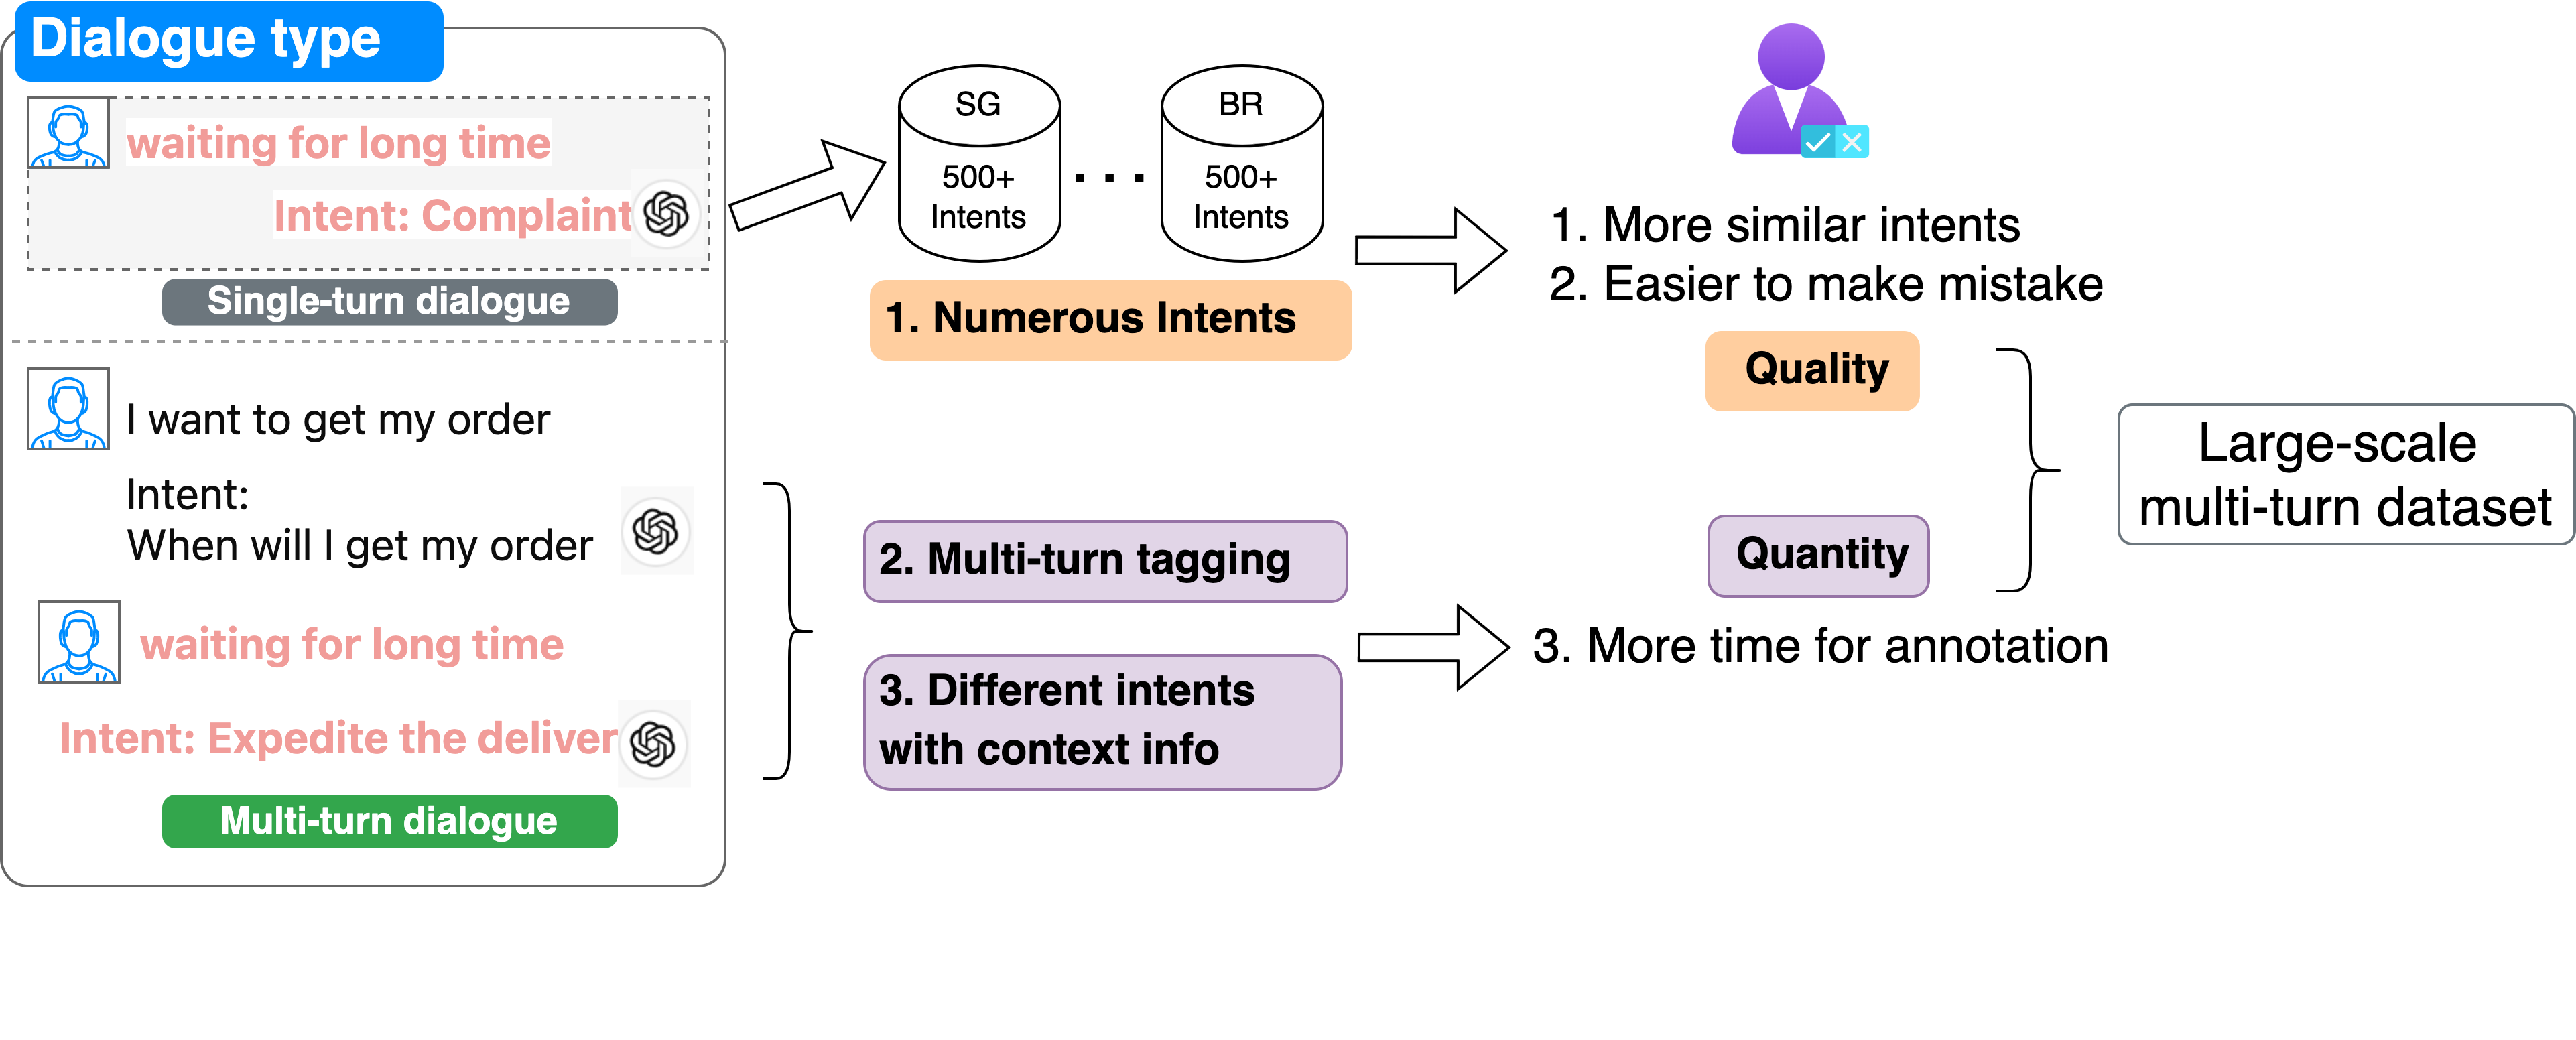
\includegraphics[width=.95\textwidth]{Figures/Challenge-for-multi-turn-dialogue.png}
    \vspace{-1cm}
    \caption{Annotation pipeline of multi-turn intent classification dataset }
    % \caption{Annotation pipeline of multi-turn intent classification dataset - a challenging task as there are hundreds of intents within the knowledge base of a chatbot to cover users' specific intents for each market. Furthermore, the complexity of classification increases as the number of market increases. }
    \label{fig:challenges}
    \vspace{-0.3cm}
\end{figure*}

The biggest challenge is that multi-turn datasets are hard to collect. %Some studies have already been done on this problem of 
While there are some studies on dialogue understanding in multi-turn intent classification~\cite{9082602,wu2021contextaware,Qu_2019}, they are made under the assumption of the availability of multi-turn training data, which is usually not the case in the real world. 

Figure~\ref{fig:challenges} shows the annotation pipeline of multi-turn intent classification. Unlike emotion recognition in conversation (ERC) with only less than 10 classes or topic classification within dialogue state tracking (DST) with tens of topics, there are hundreds of intents within the knowledge base of a chatbot to cover users' specific intents in each market, which increases the complexity of classification tasks and multi-turn data annotation. Annotators can easily make mistakes and spend more time making decisions due to the numerous intents. Combined, these make it a high-cost and time-consuming annotation task, and it is unrealistic to annotate large-scale multi-turn datasets manually. However, the performance will most likely suffer without enough training sample size. This calls for a more efficient method in solving the challenge \cite{Mo2023LearningTR}. 

%In this paper, we first study the feasibility of using LLM for supervised fine-tuning (SFT) to perform multi-turn intent classification using a generative method. Various intents increase the complexity of this task since the more tokens a large language model(LLM) generates, the lower the task performance \cite{rust2021good}. To conquer this, we showed two techniques: 1) compressed generation and 2) cross-lingual label, which help to reduce the difficulty of multi-turn classification tasks using the LLM generative method. 


%When building a transnational application, we also need to cope with the language understanding of different markets. Besides, there are also distinct intent sets which are catered to the local business operations, and the intents are ever changing over the course of business. Manually annotating and maintaining large scale multi-turn dataset is simply unrealistic. 

To tackle the above challenge, we propose \textbf{L}inguistic-\textbf{A}daptive \textbf{R}etrieval-\textbf{A}ugmentation, or LARA, which offers a pipeline of techniques to adopt only single-turn training data to optimize multi-turn dialogue classification. LARA first leverages an XLM-based model trained on single-turn classification datasets for each market, thus simplifying data construction and maintenance. Subsequently, LARA advances the field by selecting plausible candidate intents from user utterances and employing a retriever to gather relevant questions for prompt construction. This process facilitates in-context learning (ICL) with multi-lingual LLMs (MLLMs), significantly enhancing model efficacy without requiring market-specific multi-turn models.

% Firstly, we trained an XLM-based model on our single-turn classification dataset of each market, which is easier to construct and maintain. Secondly, the model can classify plausible candidate intents from all utterances from the user side. Then we adopt a retriever to collect 9 most similar questions under those candidate intents. Finally, we construct prompts based on them  and feed them into multi-lingual LLM (MLLM). With MLLM, we also relax the requirement to train multi-turn models for each market. 

In summary, the contributions of this paper are as follows:

%In this method  using LLM through in-context learning (ICL) in a zero-shot setting. To overcome the context limit of LLMs involving many intents, we introduced a way to retrieve highly plausible candidate intents using a single-turn model, which also helped filter noises for in-context learning.

\begin{enumerate}
  \item We introduce LARA as a multi-turn classification model only leveraging single-turn datasets to effectively address multi-turn data collection issues. 
  \item We conduct experiments on our e-commerce multi-turn dataset across six languages. LARA achieves state-of-the-art results and reduces inference time during ICL with MLLMs.
\end{enumerate}

\section{Related Work}
% \subsection{Intent Classification}
% Intent classification is a typical text classification task where class labels are intent names. Various neural networks have inspired a wide range of studies aimed at creating neural models for text classification. Various neural model structures such as CNN \cite{conneau2016very,kim-2014-convolutional}, LSTM \cite{yang2016hierarchical} and GCN \cite{yao2019graph,liu2024spatial} have proven more effective than conventional methods. Additionally, some studies \cite{zhang2017multi,zhang2020multi} utilize label embeddings and train them simultaneously with the input texts. In recent developments, the accomplishments of large-scale pre-training language models (PLM) \cite{kenton2019bert} have generated significant interest in incorporating this pre-training approach \cite{reimers2019sentence} into monolingual and multilingual text classification \cite{conneau2020unsupervised}. However, most works are single-turn text classification tasks, which is unsuitable for multilingual multi-turn intent classification.

\textbf{Modeling Multi-turn Dialogue Context}: Modelling the multi-turn dialogues is the foundation for dialogue understanding tasks. Previous works adopt bidirectional contextual LSTM \cite{ghosal2021exploring,liu2022title2vec} to create context-aware utterance representation on MultiWOZ intent classification \cite{budzianowski2018multiwoz}. Recent works use PLM as a sentence encoder \cite{shen2021directed} on emotion recognition in conversation (ERC). Specifically, \cite{lee2022compm} used PLM to encode the context and speaker's memory and \cite{qin2023bert} enhance PLM by integrating multi-turn info from the utterance, context and dialogue structure through fine-tuning. However, all of their tasks adopt the multi-turn dialogue training set, which is hard to collect for an e-commerce chatbot. Our method attempts to combine an XLM-based model trained on the single-turn dataset into an in-context retrieval augmented pipeline with LLM, solving the multi-turn intent classification task in a zero-shot setting. 

%\subsection{In-context learning and Retrieval Augmented Generation}
% will link the references later
%In-context learning has become successful with the Large language model and has changed the approach to text classification. Not like fine-tuning, struggles when the number of available training samples is limited \cite{dodge2020fine}. The scarcity of contextual multi-turn dialogue interaction further calls for the need of methods which do not rely on expensive training data curation. \cite{brown2020language} has shown that large-scale language models performs competitively in many NLP tasks through in-context learning (ICL), even when no explicit training on the task was done. Recent work \cite{milios2023context} has applied ICL to a classification task with many labels. In this approach, demonstrations are dynamically retrieved to fit within the model's context window. Our work diverges from this in that the demonstrations in the context are not precisely aligned with the target task; while the demonstrations focus on single-turn intent recognition, the target task involves multi-turn intent recognition. However, \cite{cheng2023uprise} has also demonstrated that even when the demonstrations do not precisely match the target task, they can still aid in model inference, especially if they are closely related.

\noindent\textbf{In-context Retrieval}: In-context learning (ICL) with LLM like GPT-3 \cite{gpt3} demonstrates the significant improvement on few-shot/zero-shot NLP tasks. ICL has been successful in utterance-level tasks like intent classification \cite{Yu2021FewshotIC}. As for the \textbf{Retrieval} part, most research on in-context learning (ICL) usually deals with single sentences or document retrieval, but we are interested in finding and understanding dialogues. Generally, there are two types of systems to find the relevant dialogues: the first is LM-score based retrieval. They \cite{Rubin2021LearningTR, Shin2021ConstrainedLM} check the probability of a language model, like GPT-3, to decode the right answer based on an example. The second type defines similarity metrics between task results and uses them as the training objective for the retriever. Both K-highest and lowest examples are used as positive and negative samples to help the system learn. The most pertinent research on dialogue retrieval concentrates on areas such as knowledge identification \cite{Wu2021DIALKIKI} and response selection \cite{Yuan2019MultihopSN}. Our objectives and settings differ from them.
 % \boldsymbol{Multilingual LLM}
 % \boldsymbol{ In-context learning （RAG）}
 % \boldsymbol{Text Classification with LLM}
\section{Problem Formulation}

% \subsection{The Challenges}

% Research in multi-turn intent recognition has predominantly focused on modeling strategies. However, a critical challenge often overlooked is the scarcity of annotated, application-specific multi-turn datasets. Publicly available datasets typically encompass a limited number of intents, generally in the tens, which does not reflect the complexity encountered in real-world applications requiring hundreds of intents to accurately respond to user needs. The necessity for large-scale, annotated training datasets for effective model performance is evident, yet the dynamic nature of intent lists in ongoing business operations complicates dataset maintenance due to frequent updates and expansions of intent categories.

% Furthermore, the annotation process for multi-turn conversations is considerably more complex and error-prone than that for single-turn interactions. This complexity arises from the nuanced roles of context in conversations, including dependencies such as system responses influencing subsequent user queries. These factors contribute to potential semantic drifts over time and complicate the training data curation process, especially when considering the need for multi-lingual support.

% \subsection{Single-turn vs. Multi-turn Intent Recognition}
\subsection{Hierarchical Text Classification}
Hierarchical text classification (HTC) is a type of text classification where the classes or categories are organized in a hierarchy or tree structure. Instead of having a flat list of categories, the categories are arranged in a nested manner, so we need to consider the relationships of the nodes from different levels in the class taxonomy. 
% However, methods which optimally utilise the overall label hierarchy information often outperform the methods which simply disregard the structure and treat them as flat text classification, as they can take advantage of the extra information. \cite{Rojas2020EfficientSF}

The intents in our scenario are organised in a hierarchical tree structure. Specifically, each category can belong to at most one parent category and can have arbitrary number of children categories. Our class taxonomy $\mathcal{T}$ is a tree with fixed depth 3 and one meta root node, that is, the distance from the root node to all leaf nodes is 3, and the unique path from the root node to each leaf node will form one intent. 

We formulate the single-turn HTC task in our scenario as such, given a text $q_i$, the purpose is to predict a subset $I$ of the complete intent set $\mathcal{I}$, where the size of the subset $|I|$ containing the category from each layer is 3 (excluding root node). Generally, the number of intent sets exceeds 200.  

% \subsection{Single-turn Intent Classification} In the single-turn scenario, the objective is to classify a user's query $q$ into one of the predefined intent set $|I|$ from $\mathcal{I}$, where $|\mathcal{I}|$ often exceeds 200. Queries are complete and meaningful texts ranging from informational requests to action-oriented dialogues. Recognizing the correct intent enables the dialogue system to provide relevant solutions or perform specific actions. This process is further complicated in transnational applications that must accommodate queries in multiple languages and adapt to localized business operations.

\subsection{Multi-turn Intent Classification} Multi-turn scenario shares the same $\mathcal{T}$ and $\mathcal{I}$ as single-turn scenario. It involves a series of user queries $\mathcal{Q} = \{q_i\}_{i=1}^n$ in dialogues, the objective is to identify the intent of the final query $q_n$. Multi-turn recognition must account for the entire conversational context $\mathcal{C} = \{q_i\}_{i=1}^{n-1}$, which includes the historical queries. This context-dependency introduces additional complexity, requiring models to interpret nuanced conversational dynamics and adjust to evolving user intentions over the course of an interaction.

\subsection{Objective} This work aims to use easily accessible single-turn data to improve the accuracy of multi-turn intent recognition without requiring any multi-turn training datasets. 

% By proposing LARA that dynamically adapts to the conversation's context while minimizing reliance on large-scale annotated multi-turn datasets, we seek to mitigate the significant annotation challenges and enable more effective intent recognition in complex multi-turn dialogues.


% \subsection{Multi-turn Intent Recognition}
% While studies have been done on the multi-turn intent recognition, the focus is mainly on the modelling part. We argue that the most practical aspect of the task, which is the absence of annotated application-specific multi-turn dataset, is ignored. Moreover, the public datasets only have very few intents, usually on the scale of tens. When facing a real-life scenario where several hundreds of intents are needed to cater to users' need, a large scale annotated training dataset is needed for the supervised finetuned model to perform adequately good. One previous work \cite{Liu2020EnhancingMD} has considered the curation of large scale domain-specific multi-turn training data spanning a large number of intents. However, it requires manual annotation of 600k multi-turn sessions firstly to train a model to automatically annotate the remaining 400k sessions, making up to 1M samples in total. Considering that for an on-going business, the intent list will most likely change from time to time, e.g. some existing intents might be further broken down into more granular ones, and this will require re-annotation of part of the massive dataset.

% On the other hand, in single-turn intent recognition, the training data is easier to be constructed and maintained. This is due to there only exists one query and intent pair for each training sample. The complex behaviour and roles of context in a multi-turn conversation \cite{ghosal-etal-2021-exploring} makes the annotation process difficult and tricky. There are also other dependency possibilities to be considered for inclusion such as the influence of system answer on the next user query, i.e. the solutions shown are important for context understanding, but they might change over time, causing the possible user follow-up queries to change, and hence a semantic drift in the future. Not to mention about the dimension of query languages, which will need more annotated samples for training. In this work, we aim to find a relatively hassle-free method with strong performance which only extends from the available single-turn training data. 

% In the remaining subsections, we will formulate the problem for the ease of further discussions.

% \subsubsection{Single-turn Intent Recognition} In a single-turn scenario, given a user query $q$, the goal is to recognize the user intention from a list of intent classes $\mathcal{I} = \{I_i\}_{i=1}^k$, where $k$ is usually more than 200. A query could be an answer-seeking question like enquiries about the payment methods supported, or a task-oriented dialogue like order cancellation. By recognizing the intent, the dialogue system can help to provide the solution or perform the action accordingly. In a transnational business application, the model is expected to handle queries in multiple and mixed languages. The intent list $\mathcal{I}$ for each market could be also different to cater to the local business operations. In our scenario, each intent $I$ comprises $\langle r, l \rangle$ where $r$ is a representative query for the intent in the local language, and $l$ is the hierarchical label names in English (``\emph{Product} $>$ \emph{intention}", e.g. ``Food $>$ Cancel order", ``Digital Product $>$ Cancel order", ...).

% % \subsection{What’s single-turn/multi-turn intent recognition task}
% \subsubsection{Multi-turn Intent Recognition} In a multi-turn conversation scenario, we are given a conversation session corresponding to a sequence of queries, i.e., $\mathcal{Q} = \{q_i\}_{i=1}^n$. The goal is to recognize the user intention for the last query $q_n$. Each query turn can be ambiguous and is usually context-dependent, thus we need to consider the conversational context $\mathcal{C}$ when recognizing the user's true intention. Two types of context $\mathcal{C}$ are considered in the methods to be presented: (1) The context containing historical queries and the corresponding ground truth intent $\mathcal{C}_{\mathcal{Q}\mathcal{I}^*} = \{q_i, I^*_i\}_i^{n-1}$ and (2) containing historical queries only $\mathcal{C}_{\mathcal{Q}} = \{q_i\}_i^{n-1}$. During inference time, when the ground truth $I^*_i$ is not known, it is replace with the model prediction for that corresponding turn. 

% Both single-turn and multi-turn share the same intent classes $\mathcal{I}$. We assume that the training data $\mathcal{D} = \{\langle x_i, y_i\rangle\}$ for single-turn intent recognition, where $y_i \in \mathcal{I}$, is readily available as it is easier to be curated compared to its multi-turn counter part, and a traditional classification model $\mathcal{M}_c$ is trained on the dataset $\mathcal{D}$.

\begin{figure*}[t]
    \centering
    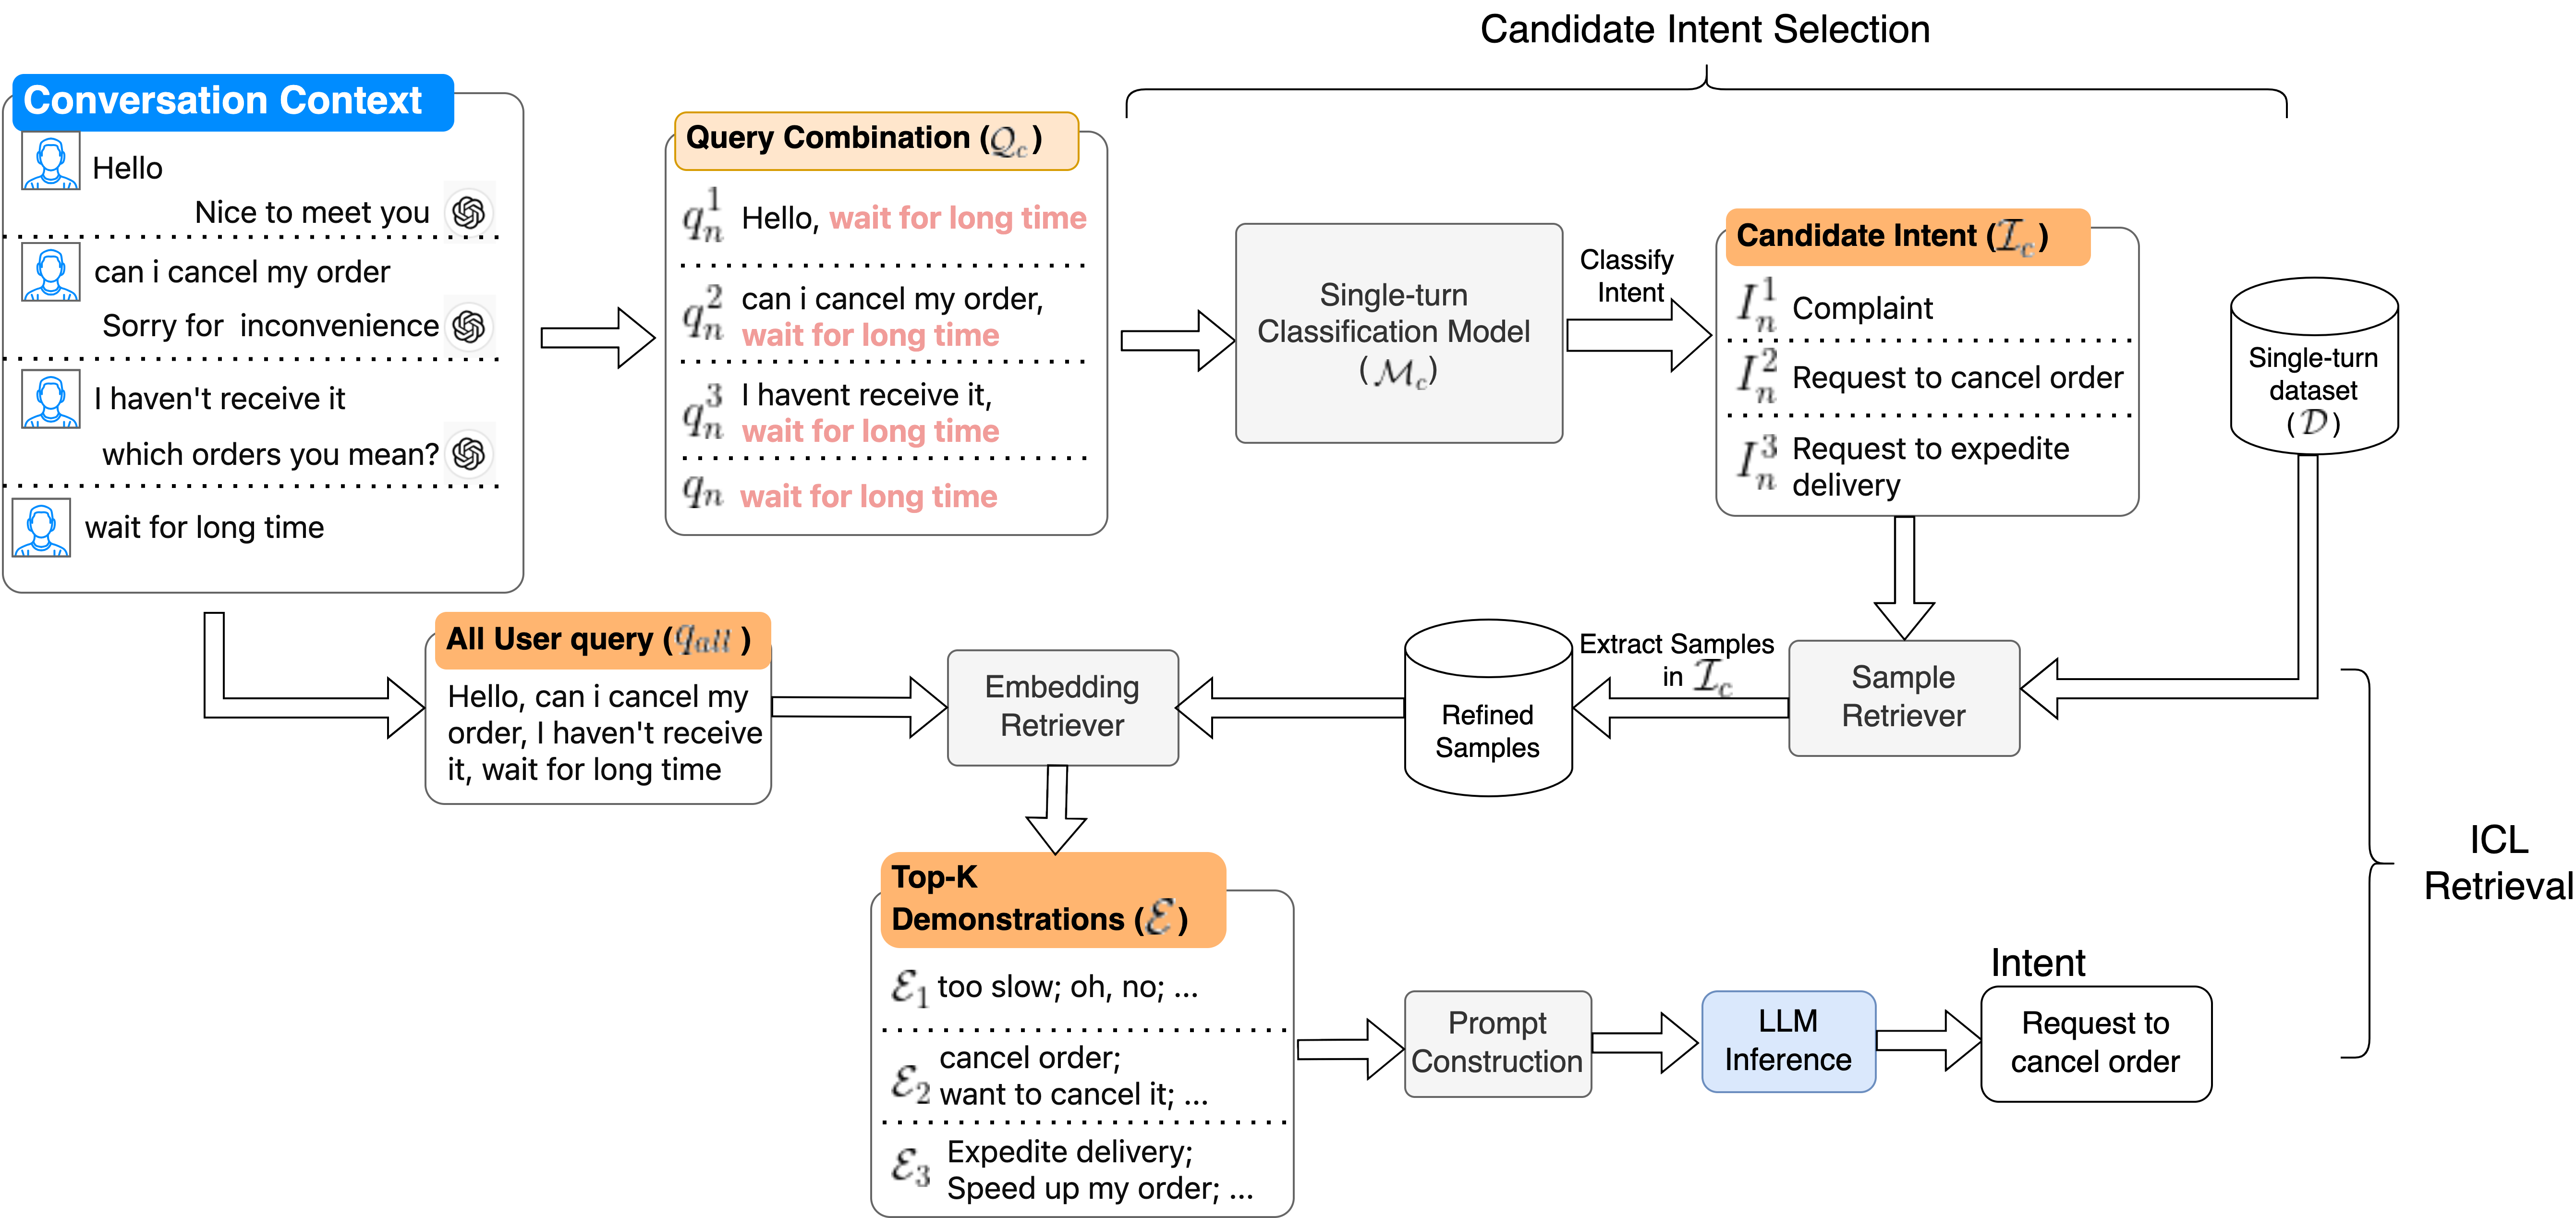
\includegraphics[width=.9\textwidth]{Figures/LLM_in_ICL_way.png}
    \caption{The pipeline of Linguistic-Adaptive Retrieval-Augmentation}
    \label{fig:ICLway}
    \vspace{-0.2cm}
\end{figure*}

\section{LARA: Linguistic-Adaptive Retrieval-Augmentation}



% \subsection{ Supervised Fine-tuning with LLMs }

% % Before delving into LARA, which is the focus of this work, we first consider the supervised finetuning approach. Unlike any other discriminative or regressive methods, we frame this task as a generative one with LLM as the foundation. That is, given the $q_n$ and its context $\mathcal{C}_{\mathcal{Q}\mathcal{I}}$, where the queries and intents are represented in a natural question answering flow of a conversation session $\{q_1, r_1, ..., q_{n-1}, r_{n-1}, q_n\}$, the model is trained to generate the corresponding representative question $r$ of the correct intent $I$ for $q_n$. The complete model input prompt can be found in the appendix. 

% As the Multi-turn Intent Recognition task is formulated as a generative problem, the use of LLMs with suprevised Fine-tuning (SFT) form the foundational approach. Concretely, given the query $q_n$ and its context $\mathcal{C}_{\mathcal{Q}\mathcal{I}}$, where queries and intents follow a natural question-answering flow within a conversation session $\{q_1, r_1, \ldots, q_{n-1}, r_{n-1}, q_n\}$, a model is trained to generate the intent representative query $r$ corresponding to the correct intent $I$ for $q_n$~\footnote{Details on model input prompts are provided in the appendix.}.


% \subsubsection{Compressed Generation} 
% % The representative query $r$ of each intent has on average 12 tokens and are ill-suited to be used as generation labels. The excessive information from the combination of those token count would be wasted considering the number of intents we have, and be unnecessarily complex for model learning. As such, ChatGPT-3.5-turbo is used to compress each $r$ into 2 words in the same language preserving the definition, whereby each intent will be ensured to have different $r_{compressed}$. One of the examples of compressions would be ``How to schedule the date and time of delivery for my order?" $\rightarrow$ ``Order scheduling", where the superfluous information is removed. The compression will start from $r$ with the least words, the logic being that the shorter $r$ will contain less information. If a collision happens after compression, i.e. the new $r_{compressed}$ has been seen before, the ChatGPT-3.5-turbo model will be prompted to compress it again with final word counts increased by 1, until a new $r_{compressed}$ is obtained. After the process, the resulting $r_{compressed}$s have on average 4 tokens. 
% Given that the intent representative query $r$ averages 12 tokens and is thus unsuitable for generation labels, a LLM is employed to condense each $r$ into two words in the same language while preserving the intent's essence, ensuring unique $r_{compressed}$ for each intent. This process begins with the shortest $r$, under the premise that shorter $r$ contains more focused information. In case of duplicate $r_{compressed}$, the model iterates the compression, incrementally increasing word count until uniqueness is achieved, resulting in $r_{compressed}$ averaging four tokens.


% \subsubsection{Cross-Lingual Labels} 

% % For non-English markets, we also tried to compress $r$ into English, keeping $\mathcal{Q}$ in the original language. English is the major language in LLMs pretraining corpus, generating labels in a language they are stronger in could pose lower difficulty.

% For non-English content, $r$ is also compressed into English while maintaining $\mathcal{Q}$ in the original language, leveraging English's prevalence in LLM pretraining corpora to potentially simplify label generation.


The LARA framework shown in Figure \ref{fig:ICLway} addresses the multi-turn intent recognition challenge through zero-shot in-context learning with single-turn demonstrations guided by a crafted instruction prompt. First, a single-turn classification model $\mathcal{M}_c$ is trained on single-turn dataset and used to narrow down the intents to be included in the ICL prompt, which are henceforth referred to as candidate intents. This step is necessary due to the limited LLM context window, and it also helps to filter out extra noise from direct demonstration retrieval. Then, for every candidate intent, in-context demonstrations are selected by retrieving single-turn examples that are semantically similar to the multi-turn test sample. Finally, an instruction prompt for multi-turn classification is formulated by combining the demonstrations and test user queries.


\subsection{Single-turn Classification Model ($\mathcal{M}_c$)}
Before diving into LARA, we must train a single-turn hierarchical text classification model on our single-turn dataset $\mathcal{D}$. The model is an ensemble of a simple label-attention model \cite{zhang2020multi} and a state-of-the-art HTC approach named HiTIN \cite{Zhu2023HiTINHT}. The label-attention model only considers the semantic info of user utterances and label-query attention info, which ignores the hierarchical tree-like structure in our intent system. So, we build model $\mathcal{M}_c$, integrating taxonomic structure via the tree isomorphism network within HiTIN into our label-attention model. More details are provided in Appendix \ref{appendix:a}.

We conduct some experiments on our multilingual dataset. The result in Table \ref{table:htc_improvement} shows that HiTIN alone performs better than the label-attention model, and ensembling the two methods further improves performance on average scores. We will use this model as our baseline and generate candidate intents within LARA.

% The ensemble model forms a strong baseline compared to the flat approach used in the LARA pipeline, which is unaware of the taxonomic hierarchy during the in-context learning process. Hence, the effectiveness of LARA is shown even when compared to a non-basic method.

\begin{table*}[t]
\centering
\scalebox{0.8}{
\begin{tabular}{||l c c c c c c c c c||} 
 \hline
  & BR & ID & MY & PH & SG & TH & TW & VN & avg \\ [0.5ex] 
 \hline\hline
 Traffic weight & 150k & 212k & 27k & 46k & 5k & 36k & 36k & 43k &  \\
 \hline\hline
 Label-attention model & 81.55\% & 87.91\% & 83.73\% & 73.29\% & 83.69\% & 83.11\% & 71.55\% & 74.44\% & 82.30\% \\
 HiTIN & 81.85\% & 89.41\% & 84.57\% & 74.75\% & 84.17\% & 83.67\% & \textbf{75.38}\% & \textbf{75.99}\% & 83.53\% \\
 Ensembled  & \textbf{82.66}\% & \textbf{89.62}\% & \textbf{85.33}\% & \textbf{75.98}\% & \textbf{84.57}\% & \textbf{83.89}\% & 75.19\% & 75.52\% & \textbf{83.94}\% \\[1ex]
 \hline
\end{tabular}}
\caption{Noticeable improvement from adding a state-of-the-art HTC approach.} 
% Ensembling two different methods further improved the performance. The averages are aggregated by traffic weight. }
\vspace{-0.2cm}
\label{table:htc_improvement}
\end{table*}


\subsection{Candidate Intents Selection}
\textbf{Query Combination}: After receiving the context from user side, the last query $q_n$ is first combined with each historical query in conversational context $\mathcal{C}$ to form a query combination set $\mathcal{Q}_c$ = $\{q_n, q^1_n, ..., q^{n-1}_n\}$, where $q^i_n$ means the text concatenation of $q_i$ with $q_n$ using a comma. 

\noindent\textbf{Candidate Intent Recognition}: $\mathcal{M}_c$ predicts few candidate intents $\mathcal{I}_{c}$ from all intents $\mathcal{I}$ on these query combinations $\mathcal{Q}_c$. The $\mathcal{M}_c$ is then used to perform inference on each of the concatenated queries to get a set of candidate intents $\mathcal{I}_{c} = \{I_{q_n}, I_{q^1_n}, ..., I_{q^{n-1}_n}\}$. Finally, we will select the top 3 intents with the highest scores. Note that $\mathcal{I}_{c}$ is a set, so duplicated intents will be removed, and the maximum size of $\mathcal{I}_{c}$ is equal to the number of queries $n$ in a session. 


% \subsection{Candidate Intents Selection}
% In terms of candidate intents selection, not all intents from $\mathcal{I}$ are incorporated into the ICL prompt. Instead, the single-turn classification model $\mathcal{M}_c$ narrows down to a subset of candidate intents $\mathcal{I}_{candidates}$, derived from combining the last query $q_n$ with each historical query in $\mathcal{C}_{\mathcal{Q}}$, forming $\mathcal{Q}_{combinations}$. The model's inference on these combinations yields $\mathcal{I}_{candidates}$, a set removing duplicates with its size, $M$, equating to the session's query count $n$.

% Do note that the combination of the top intents from each $P_l$ might not be a valid intent in the intent taxonomy. Hence, we perform one extra step of beam search decoding on the 3 layers results to get a valid top intent. The selection process is detailed in Appendix \ref{appendix:a.1}.

\subsection{ICL Retrieval}
% For each unique $\mathcal{I}_{candidates}^m$ in $\mathcal{I}_{candidates}$, we retrieve top $K$ $\langle x_i, y_i\rangle$ with $y_i \equiv \mathcal{I}_{candidates}^m$ according to the cosine similarity of $x_i$ to the concatenation of all the queries in conversation $q_{all} = q_1 \circ ... \circ q_{n-1} \circ q_n$. We then have a single-turn task demonstration collection $\mathcal{E} = \{ \{s(x_k^m, y_k^m)\}_{k=1}^K; y^m \equiv \mathcal{I}_{candidates}^m \}_{m=1}^M $ of size $M \times K$, where $s(x_k, y_k)$ is a demonstration written in natural language texts with a sample query $x_k$ and the English hierarchical label name $l$ of its corresponding $y_k$. The retrieval model used is a domain sentence encoder pretrained to be able to retrieve text based on cosine similarity of the embedding vectors it produces. 

% Demonstrations are retrieved from the single-turn dataset for each intent in $\mathcal{I}_{candidates}$. Demonstrations consist of a sequence of annotated examples:
% \begin{displaymath}\{(x_{demo}^1, y_{demo}^1), ..., (x_{demo}^k, y_{demo}^k)\}\end{displaymath}
% where $x_{demo}^j$, $1 \leq j \leq k$ denotes the $j$th single-turn sample query and $y_{demo}^j$ denotes the text representing the label, which in our case is the English hierarchical label name $l$. Demonstrations serve two purposes: (1) provides the LLM with evidence to consult on for decision making, i.e. intents and their example queries content; (2) Specifies an output format that LLM outputs must adhere to, thereby enabling straightforward transformation of the model output in natural language into labels.

However, not all training examples under the candidate's intent $\mathcal{I}_{c}$ will be used in the prompt as demonstrations. Here, the demonstrations refer to a sequence of annotated examples that provide LLM with decision-making evidence and specify an output format for natural language conversion into labels during ICL. Our strategy is to sample training examples that are similar to the test sequence for each candidate intent, a method introduced by \cite{liu2021makes}. In this process, we first concatenate all the queries in the session with a comma to get the test sequence $q_{all}$. Then, $q_{all}$ is mapped to a vector $H_{q}$ using the [CLS] token embedding from a pre-trained sentence encoder, $\Phi_{XLMR}$. After that, we retrieve all the single-turn training samples for each candidate intent from $\mathcal{D}$ using a sample retriever and also encode them using $\Phi_{XLMR}$. With $H_{q}$ as query, we use an embedding retriever to search through the sampled examples to retrieve top $K$ - 1 nearest data examples of each candidate intent based on their cosine similarity to $H_{q}$. Together with the representative query of each candidate intent, the retrieved single-turn samples of all candidate intents form the demonstrations $\mathcal{E}$ for in-context learning. We show the detailed algorithm in \ref{alg:retrieval} below.
 % = \{x_j, y_j\}_{j=1}^{K \times M}



\subsection{Prompt Construction and LLM Inference}
% A multi-turn intent recognition task instruction $\mathcal{T}$ is hand-crafted to guide the model to perform multi-turn intent recognition task by referring to the single-turn demonstrations. The complete input prompt $\mathcal{P} = \{\mathcal{T}, \mathcal{E}, \mathcal{C_{\mathcal{Q}}}, q_n\}$ will consist of the task instruction, single-turn demonstrations, context, and the last query. These components are concatenated together to form a text sequence. One point to note is that, the demonstrations in $\mathcal{E}$ are sorted in ascending order based on their cosine similarity scores to $q_{all}$, regardless of intent. This is due to the sensitivity of LLM ICL to their 

% Taking into account the inference speed requirement of real-time applications, we tried two extra methods to constraint the model to generate only a single-token symbol, unique to each intent. (1) $\mathcal{P}_{symbolic} = \{\mathcal{T}_{symbolic}, \mathcal{E}_{symbolic}, \mathcal{C_{\mathcal{Q}}}, q_n\}$. The original label name $l$ of each $y_j$ in $\mathcal{E}_{symbolic}$ are replaced with single-token symbols, e.g. `A', `B', ..., which bears no meaning to the intents they represented. Explanation will be made in the instruction prompt $\mathcal{T}_{symbolic}$ to link the symbols back to their original intent label $y_j$, and the model is instructed to generated the symbols instead of full label names; (2) $\mathcal{P}_{prepend} = \{\mathcal{T}, \mathcal{E}_{prepend}, \mathcal{C_{\mathcal{Q}}}, q_n\}$. In $\mathcal{E}_{prepend}$, representative symbols for each intent will be prepend to the original label name $l$, such that they are separated by an extra character as boundary, e.g. label ``Food $>$ Cancel order" will be written as ``A $>$ Food $>$ Cancel order" in the prompt. Note that the instruction prompt $\mathcal{T}$ remains the same, the trick is to limit the model generation token count to 1 on API level, such that only the symbols `A', `B', ... will be generated. A map from each symbol to their respective intent will be kept when constructing the prompt. Finally, model outputs are greedily decoded, ensuring efficient and accurate intent recognition. An example of each $\mathcal{P}$ variant can be found in the appendix. 
% To include the conversational context $\mathcal{C}$ into the prompt, we need to concatenate all historical questions into one single text. This is achieved by first adding additional semantic prefixes "[History msg {i}] " to each historical question, where $i \in \{1, ..., n-1\}$, before concatenating them with new line characters. For $\mathcal{E}$, . 
A task instruction $T$ is hand-crafted to guide the model to perform multi-turn intent recognition task by referring to the single-turn demonstrations. The task instruction $T$, combined with demonstrations $\mathcal{E}$, conversational context $\mathcal{C}$, and the query $q_n$, forms the input prompt $\mathcal{P}$ for the LLM. The concatenation of each prompt component into one long text is shown in the appendix \ref{appendix:c}. To accommodate real-time application latency requirements, two additional methods were explored to constrain the model to generate single-token symbols representing intents, detailed as $\mathcal{P}_{symbolic}$ and $\mathcal{P}_{prepend}$, with examples also provided in the appendix. Model outputs are greedily decoded, ensuring efficient and accurate intent recognition.

% \section{Algorithm for ICL Retrieval}
% \label{appendix:c}
% \subsection{Algorithm for Candidate Intent Selection}
% \label{appendix:a.1}

% % TODO: beam search? Wont they question the use of beam size?
% \begin{algorithm}[t]
% \caption{Candidate Intent Selection}\label{alg:candidate_selection}
% \begin{algorithmic}
% \let\oldReturn\Return
% \renewcommand{\Return}{\State\oldReturn}
% \Require {$ \mathcal{Q}_c = \{q_n, q^1_n, ..., q^{n-1}_n\} $}
% \For { each item $q_i$ in $\mathcal{Q}_c$ }
%   \State Get $P_1$, $P_2$, $P_3$ for all three layers from $\mathcal{M}_c(q_i)$
%   \State
%   \State Perform beam search with beam size 5 on $P_1$, $P_2$, $P_3$ to obtain top 1 valid intent $I_i$ in taxonomy
%   \State
% \EndFor
% \Return $ \mathcal{I}_{c} = \{I_n, I^1_n, ..., I^{n-1}_n\} $
% \end{algorithmic}
% \end{algorithm}

\begin{algorithm}[t]
\caption{ICL Demonstrations Retrieval}\label{alg:retrieval}
\begin{algorithmic}
\let\oldReturn\Return
\renewcommand{\Return}{\State\oldReturn}
\Require $\mathcal{I}_c$, $Q$, a positive integer $K$
\State $ \mathcal{I}' = remove\_duplicate(\mathcal{I}_c) $
\State $ q_{all} = text\_concatenate(\mathcal{Q}) $
\State $ H_q = \Phi_{XLMR}(q_{all})^{[CLS]} $
\State
\For { each item $I_i$ in $\mathcal{I}'$ }
  % \State $ X_i = get\_training\_samples\_from\_\mathcal{D}\_for\_intent(I_i) $
  \State /* Sample retriever: Get the single-turn training samples under intent $I_i$ */
  \State $ X_i = sample\_from\_\mathcal{D}\_for\_intent(I_i) $
  \State
  \State /* Embedding retriever: Get embedding for each training sample */
  \State $ H_{X_i} = \{\Phi_{XLMR}(x_j)^{[CLS]}\}_{j=1}^{|X_i|}, x \in X_i $
  \State
  \State /* Calculate text similarity of each training sample with test queries */
  \State $ S_i = \{cosine\_similarity(H_q, h_j)\}_{j=1}^{|H_{X_i}|}$, where $h \in H_{X_i} $
  \State
  \State /* Get top $K$ nearest demonstrations */
  \State $ \mathcal{E}_i \gets $ Top $ (K-1) $ $ x \in X_i$ based on $S_i$
  \State Append $r$ of $I_i$ to $\mathcal{E}_i$ /* add representative query to demonstrations of $I_i$ */
\EndFor
\State
\State $ \mathcal{E} = \{\mathcal{E}_i\}_{i=1}^{|\mathcal{I}'|} $ /* collect demonstrations of all candidate intents */
\State $ S = \{S_i\}_{i=1}^{|\mathcal{I}'|} $
\State Sort $ \mathcal{E} $ by their scores $S$ in ascending order
\State
\Return $ \mathcal{E} $
\end{algorithmic}
\end{algorithm}
\section{Experiments}
\subsection{Experimental Setup}
\textbf{Dataset}. The dataset is obtained from the conversation history of a large e-commerce company. It consists of user queries in the local languages of eight markets: Brazil, Indonesia, Malaysia, Philippines, Singapore, Thailand, Taiwan, and Vietnam.  All the labelled data are collected through manual annotation by local customer service teams of each market. The samples with consistency labels from 3 taggers are selected to ensure the annotation quality. More details are in Appendix \ref{appendix:b}.



\noindent\textbf{Metrics}. We evaluate the accuracy of the methods based only on the label of the last query $q_n$ in each conversation session $\mathcal{Q}$. Other metrics which consider class imbalance are not used as the sampled sessions are expected to reflect the online traffic of each intent, thus more accurately simulating true online performance.




% \begin{table}[t]
% \centering
% \begin{tabular}{||l c c c c||} 
%  \hline
%  Data Source & BR & ID & MY & SG \\ [0.5ex] 
%  \hline\hline
%  Single-Turn & 61k & 150k & 66k & 66k \\
%  Chat Log & 8k & 16k & 8k & 8k \\ 
%  Template & 37k & 37k & 37k & 37k \\ 
%  Off-Topic & 17k & 18k & 17k & 73k \\ [0.3ex] 
%  \hline\hline
%  Total & 124k & 221k & 129k & 184k \\ [0.3ex] 
%  \hline
% \end{tabular}
% \caption{Training data composition of SFT approach.}
% \label{table:data_train_sft}
% \end{table}

%  The methods used to compose the multi-turn dataset for supervised fine-tuning approach and their ratio are shown in Table \ref{table:data_train_sft}. We only tried the approach in BR, ID, MY, and SG. \textbf{Single-turn} data are sampled from the training data shown in Table \ref{table:data_train_test}. \textbf{Chat Log} data are the real user multi-turn queries that we sampled from online sessions. Undeniably, the labels of each query turn are from the single-turn model $\mathcal{M}_c$ that we deployed online, and are not fully reliable for training. Thus, for the second turn onwards, we also output another intent using the \emph{Selective expand} method that we will mention below, but at a lower concatenation threshold. When the intent is different from that of $\mathcal{M}_c$, we use vicuna-13b-v1.5 to select the more accurate intent with few-shots COT prompt. You can find the prompt used for chat log data cleaning in the appendix. In \textbf{Template} data, the transition distribution of high-frequency intents is obtained via the analysis of online sessions. Then, we sample from the distribution to get a template, and fill in each turn with the utterances which we sample from single-turn training data. Lastly, \textbf{Off-Topic} data is made up of instruction tuning samples from Alpaca and Dolly datasets, as well as some programmatically crafted queries about competitors. The purpose of this data type is to add off-topic detection ability to the model, but the ratio is then reduced in non-English markets to let the model focus more on the intent recognition task due to their lower performances. 

% \subsection{Processing Personal Data} % discuss how 


% \subsection{Metrics}



\subsection{Baselines}
Current multi-turn models are trained with multi-turn datasets, but our methods did not require such data. For a fair comparison, we adopt a state-of-the-art single-turn model mentioned in 4.1 with two types of concatenation approaches as baselines:
\subsubsection{Single-turn approach}
Inference on only the last utterance of a session using the single-turn model $\mathcal{M}_c$, all previous contexts are ignored.
\subsubsection{Naive concatenation}
All queries in a single session $\mathcal{Q}$ are concatenated using comma, and the concatenation result is fed into the single-turn model $\mathcal{M}_c$, which is enhanced by HTC approach mentioned above, for inference. HTC methods which optimally utilise the overall label hierarchy information often outperform the methods which simply disregard the structure\cite{Rojas2020EfficientSF}. 
\subsubsection{Selective concatenation}
In this approach, only one query from $\mathcal{C}_q$ is selected to be concatenated with $q_n$. The intuition is that not all history queries are helpful in understanding the last query, and the excessive use of them might introduce unwanted noise. A concatenation decision model is trained to select the most appropriate historical query. Depending on the model confidence, there might be cases where no expansion is needed at all. The concatenation result is then also fed into the single-turn model $\mathcal{M}_c$ for inference.





% \subsection{Implementation Details}
% % - models and hyperparameters
% % - context nlu and tradition model
% %    - backbone
% % - sft and icl models
% %    - learning rate, and size

% % In the LLM SFT approach, FastChat framework is used to LoRA-finetune 7B models on $q\_proj$, $v\_proj$, $o\_proj$, and $k\_proj$ modules with a learning rate of 2e-5 over 10 epochs. The 7B models used are Llama-2-7B and SeaLLM-7B-chat on Hugging Face. However, before finetuning on multi-turn intent recognition task, the Llama-2-7B base model is further LoRA-finetuned with the same setting above on a mix of ShareGPT dataset and in-domain live agent and customer chat transcript, and the weights are merged. Loss is calculated on all the model output including those after history queries. During inference, when the generated label has no exact match with any $r$ in $\mathcal{I}$, gestalt pattern matching is used to find the closest one.

% % In LARA, both 7B and 13B instruction-tuned LLMs are tested, i.e. vicuna-7b-v1.5, vicuna-7b-v1.5, and SeaLLM-7B-v2

% The traditional single-turn model, the retriever, and the concatenation decision model used are using backbone initialized with $\Phi_{XLMR}$, a multi-lingual domain specific XLM-RoBERTa-base model continued to be pre-trained with contrastive learning. We use AdamW to finetune the backbone and all other modules with a learning rate of 5e-6 and 1e-3, respectively. In LARA, the LLM used is vicuna-13b-v1.5 on Hugging Face with 13B parameters. All test are run on a single Nvidia V100 GPU card with a 32GB of GPU memory. The number of demonstrations $K$ retrieved for each intent is set at 10 in this experiment. Due to GPU memory constraint, the total number of tokens the in-context learning demonstrations can make up to are limited to 2300 tokens. If exceeded, the number of demonstrations in each candidate intent are pruned equally starting with the ones with the lowest cosine similarity scores to $q_{all}$. During inference time, if the generated intent doesn't match any of the provided options, the intent of $\mathcal{M}_c$ on $q_n$ will be considered as the final result. 
 
\section{Results and Discussions}
% \subsection{LLM SFT Techniques}
% \begin{table}[h!]
% \centering
% \begin{tabular}{||l l c c c||} 
%  \hline
%  MKT & Model & Compressed Generation & Cross-Lingual Label & Acc \\ 
%  \hline\hline
%  SG & Naive Expand & \- & \- & 60.52\% \\
%  SG & Selective Expand & \- & \- & 56.99\% \\
%  SG & Llama2-7B & 0 & 0 & 56.24\% \\ 
%  SG & Llama2-7B & 1 & 0 & 61.47\% \\
%  ID & Naive Expand & \- & \- & 60.61\% \\
%  ID & Selective Expand & \- & \- & 63.23\% \\
%  ID & SeaLLM-7B-chat & 1 & 0 & 52.49\% \\
%  ID & SeaLLM-7B-chat &1 & 1 & 55.02\% \\ [1ex] 
%  % prefix lm in ID is worse than selective expand, but better with naive expand
%  \hline
% \end{tabular}
% \caption{Performance of LLM SFT techniques.}
% \label{table:results_sft_llm}
% \end{table}
% Table \ref{table:results_sft_llm} shows the effectiveness of LLM SFT techniques introduced. Compressing the generation target lowers the difficulty of the task and significantly improves the performance. Interestingly, this technique also stopped LLM hallucination, i.e. generating label with no match in the original intent set. The hallucination rate without using compressed generation is about 2.5\%. In non-English market like ID, we find that \emph{cross-lingual label} which changes the generation target to English rather than in the local language also improved the performance. While the SFT approach performs satisfactory in English market, it still leaves a lot to be desired in non-English market.

% \subsection{LARA vs SFT}
% \begin{table}[h!]
% \centering
% \begin{tabular}{||l l c c c c||} 
%  \hline
%  Model & Prompt & BR & ID & MY & SG \\ [0.5ex] 
%  \hline\hline
%  SFT LLM &  & 48.39\% & 55.02\% & 60.83\% & 56.99\% \\
%  Vicuna-7B & $\mathcal{P}$ & 51.88\% & 60.35\% & 62.88\% & 65.26\% \\ 
%  SeaLLM-7B-chat & $\mathcal{P}$ & 51.34\% & 62.97\% & 65.00\% & 65.26\% \\ [1ex] 
%  \hline
% \end{tabular}
% \caption{In-context learning vs SFT approach.}
% \label{table:results_sft_icl}
% \end{table}
% From Table \ref{table:results_sft_icl}, we observe that in-context learning approach can outperform its SFT counterpart without going through the hassle of generating multi-turn training data which in turn might not be completely reliable. Using a multi-lingual model specific to certain markets, e.g. SeaLLM for Southeast Asia markets, can further improve the performance. 

% \subsection{LARA experiment}

% - ICL is the best methods in average
% - symbolic intent is helpless in ICL, we still need related intents within ICL
% - Symbolic answer is helpless in ICL, But can improve the RT
% - but adding historical words in message fields can further improve the performance.
Table \ref{table:results_icl} compares the performance of baselines and LARA on our multi-turn dataset. The single-turn approach has the worst performance due to the lack of context from history queries. The single-turn model with \emph{Naive concatenation} is lower than \emph{Selective concatenation} by 0.89\% on average, showing that naively including all history queries will introduce noises, which in turn jeopardizes the performance. However, pseudo-labelling the dataset used to train the concatenation decision model will need to be carefully carried out, and despite the extra steps, it will not necessarily be more effective than the naive method. 

LARA, on the other hand, with prompt $\mathcal{P}_{formatted}$, achieves the best results on most markets without any multi-turn training data. On average, it improved accuracy by 3.67\% compared with \emph{Selective concatenation}. Especially on the non-English markets, it also improved by 2.96\%, 4.18\% and 4.00\% on TH, VN and BR separately. This highlights the linguistic-adaptivity of the method on broad languages. The only market that does not outperform the baselines is ID, which most probably can be attributed to the language ability of open-sourced LLMs in handling the local slang and abbreviations in casual conversation. After all, the backbone model used in baselines is pre-trained directly on the in-domain chat log data, while the LLM models are used out of the box.


\begin{table*}[th!]
\centering
\scalebox{.8}{
\begin{tabular}{||l l c c c c c c c c c||} 
 \hline
 Model & Prompt & BR & ID & MY & PH & SG & TH & TW & VN & avg \\ [0.5ex] 
 \hline\hline
 Single-turn & - & 30.98\% & 52.14\% & 56.81\% & 40.21\% & 51.13\% & 52.99\% & 58.07\% & 65.90\% & 53.76\% \\
 Naive Concat. & - & 50.81\% & 60.61\% & 57.02\% & 47.62\% & 60.52\% & 56.97\% & 65.44\% & 76.95\% & 60.08\% \\
 Selective Concat. & - & 52.69\% & \textbf{63.23}\% & 60.20\% & 51.32\% & 56.99\% & 57.77\% & 64.02\% & 74.10\% & 60.97\% \\ 
 Vicuna-13B & $\mathcal{P}$ & 52.69\% & 61.48\% & \textbf{65.42}\% & \underline{54.50}\% & 65.26\% & 60.96\% & \textbf{67.14}\% & \underline{77.90}\% & \underline{64.18}\% \\
 Vicuna-13B & $\mathcal{P}_{symbolic}$ & 51.88\% & 60.00\% & 64.57\% & 53.97\% & 65.26\% & 58.96\% & 65.44\% & 74.67\% & 62.92\% \\
 Vicuna-13B & $\mathcal{P}_{prepend}$ & \underline{54.03}\% & 61.75\% & 64.50\% & 53.44\% & \textbf{65.94}\% & \underline{61.55}\% & \underline{66.86}\% & 75.81\% & 63.97\% \\
 Vicuna-13B & $\mathcal{P}_{formatted}$ & \textbf{55.65}\% & \underline{62.88}\% & \underline{64.71}\% & \textbf{55.03}\% & \underline{65.40}\% & \textbf{61.95}\% & \underline{66.86}\% & \textbf{78.10}\% & \textbf{64.64}\% \\[1ex]
 \hline
\end{tabular}
}
\caption{Performance of LARA compared to baselines, the average here is weighted on the number of test samples in each market. The best performance for each dataset is in boldface, while the second best is underlined.}
\label{table:results_icl}
\vspace{-0.3cm}
\end{table*}


Replacing the label names with non-related symbols in $\mathcal{P}_{symbolic}$ significantly hurts the performance of in-context learning. On the other hand, minimal changes to label names in $\mathcal{P}_{prepend}$ does not heavily impact the performance. In turn, the inference time is improved by 77\%, from 0.75it/s to 1.32it/s on a single V100 card using Hugging Face python library. Interestingly, the model also stopped generating labels which cannot be matched with the options provided in demonstrations, while previously the rate is on average 1.6\% using $\mathcal{P}$. Finally, we also tried a new prompt $\mathcal{P}_{formatted}$ based on $\mathcal{P}_{prepend}$. Only a very slight change to the context format is done, but it can outperform the other prompt variants in all datasets, suggesting that giving $\mathcal{C}_{\mathcal{Q}}$ a closer format to $\mathcal{E}$ and the targeted $q_n$ will be more beneficial in the context utilization. Besides, this also hints that the prompt could also be worked on more in the future as it is not extensively tuned in this work. 
\begin{table*}[t!]
\centering
\scalebox{.8}{
\begin{tabular}{||l c c c c c c c c c||} 
 \hline
 Encoder & BR & ID & MY & PH & SG & TH & TW & VN & avg \\ [0.5ex] 
 \hline\hline
 Our own encoder & \underline{55.65\%} & \textbf{62.88\%} & \underline{64.71\%} & 55.03\% & \textbf{65.40\%} & \underline{61.95\%} & 66.86\% & \textbf{78.10\%} & \textbf{64.64\%} \\
 
 all-MiniLM-L12-v2 & 54.57\% & 61.05\% & 64.36\% & 53.97\% & \underline{65.13\%} & 59.56\% & 68.27\% & 75.81\% & 63.63\% \\

 all-mpnet-base-v2 & \textbf{55.91\%} & 60.79\% & 63.30\% & 54.50\% & 64.31\% & 58.57\% & 67.42\% & \underline{76.95\%} & 63.24\% \\

 paraphrase-multilingual & & & & & & & & & \\
 -MiniLM-L12-v2 & 54.03\% & \underline{62.01\%} & 64.42\% & \textbf{57.14\%} & 64.31\% & \textbf{62.35\%} & \textbf{69.12\%} & \underline{76.95\%} & 64.25\%\\

 paraphrase-multilingual & & & & & & & & & \\
 -mpnet-base-v2 & 55.38\% & 61.57\% & \textbf{65.42\%} & \underline{55.56\%} & 64.99\% & 59.96\% & \underline{68.56\%} & \underline{76.95\%} & \underline{64.29\%} \\[1ex]
 \hline
\end{tabular}
}
\caption{Performance of LARA using different encoders for in-context demonstration mining. The best performance for each dataset is in bold, while the second best is underlined.}
\label{table:results_encoder}
\vspace{-0.3cm}
\end{table*}

\section{Ablation Studies}
To validate our motivation and model design, we ablate single-turn model $\mathcal{M}_c$ in candidate intent selection and retrievers in ICL retrieval. The comparison is made on the original $\mathcal{P}$ prompt variant.

\subsection{The necessity of model $\mathcal{M}_c$}
$\mathcal{M}_c$ is used to recognise the intent candidates before ICL retrieval. If so, all demonstrations are directly retrieved based on their cosine similarity to $q_{all}$ and the quality of in-context learning is adversely impacted. The accuracy on all markets dramatically dropped except PH, which only dropped by 0.53\% due to the least number of intents. The average score across all markets dropped from 64.18\% to 53.99\%. For instance, "refund timeline" and "refund timeline for cancelled order" could be confusing to retrieval-based models, while classification models trained on each market dataset can discern them better.


% As the original number of retrieved demonstrations for each $\mathcal{Q}$ is dynamic according to number of queries $n$, to ensure fairness, the number of retrieved demonstrations in this variant will also  be $ K \times n $. 
% !-- discussion to append to the part above --!
% From Figure \ref{fig:ablation}, when classification model is not used to filter candidate intents, the quality of in-context learning is adversely impacted. The performance of PH is least affected because it has the least number of intents. The larger set of intents is due to having more granular intents. For instances, "refund timeline" and "refund timeline for cancelled order", these could be confusing to retrieval-based models, while classification models trained on each market dataset can discern them better.

% \begin{table*}[t]
% \centering
% \scalebox{0.93}{
% \begin{tabular}{||l c c c c c c c c c||} 
%  \hline
%   & BR & ID & MY & PH & SG & TH & TW & VN & avg \\ [0.5ex] 
%  \hline\hline
%  Demo. pool & 66k & 161k & 74k & 33k & 76k & 60k & 31k & 178k &  \\
%  Intents & 316 & 481 & 473 & 237 & 360 & 359 & 373& 389 & \\
%  \hline\hline
%  LARA ($\mathcal{P}) $ & 52.69\% & 61.48\% & 65.42\% & 54.50\% & 65.26\% & 60.96\% & 67.14\% & 77.90\% & 64.18\% \\
%  w/o $\mathcal{M}_c$ & 46.77\% & 53.80\% & 50.81\% & 53.97\% & 58.07\% & 46.02\% & 62.61\% & 64.19\% & 53.99\% \\
%  w/o Retrieval  & 53.52\% & 60.43\% & 64.42\% & 54.44\% & 65.24\% & 60.40\% & 67.85\% & 75.35\% & 63.47\% \\
%   & $\pm$0.7\% & $\pm$0.8\% & $\pm$0.3\% & $\pm$1.3\% & $\pm$0.4\% & $\pm$0.9\% & $\pm$0.8\% & $\pm$1.3\% &  \\[1ex]
%  \hline
% \end{tabular}}
% \caption{Ablation on different components of LARA. The last row shows the standard deviations of performance `w/o Retrieval' over 10 runs. The size of the demonstration pool and the number of intents in each dataset are also included here for the ease of reference. }
% \label{table:ablation}
% \vspace{-0.2cm}
% \end{table*}

\begin{figure}[t]
    \centering
    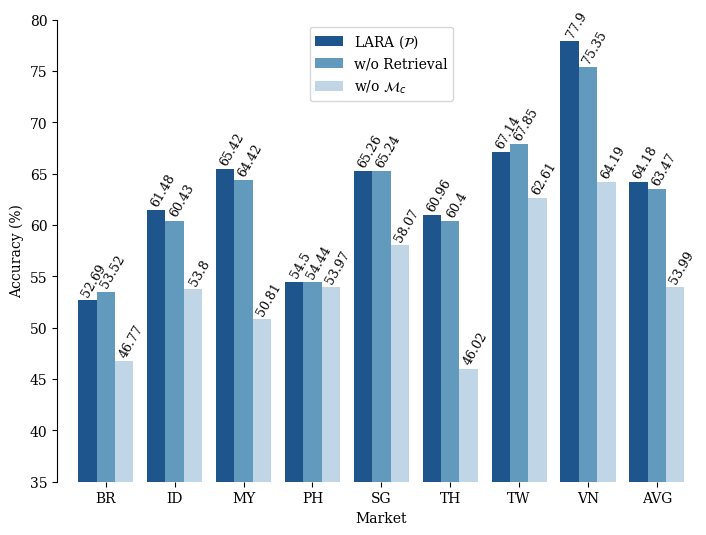
\includegraphics[width=.48\textwidth]{Figures/ablation_results.png}
    \vspace{-1cm}
    \caption{Ablation on different components of LARA.}
    \label{fig:ablation}
    \vspace{-0.3cm}
\end{figure}

\subsection{The role of retrievers in ICL retrieval}
% Demonstration selection could also have impact on the performance. Thus, we also tried to remove the retrieval component, and randomly sample the demonstrations for each intent. The results are reported with 10 runs on the random sampling. Based on Figure $\ref{fig:ablation}$, the overall performance will be worse if there is no retrieval component, specifically when there is a big demonstration pool or a high number of intents. Thus, if there is no one good strategy in pruning the demonstration pool, the easier way is to retrieval demonstrations based on their similarity to the task input.
% !-- to replace the part above --!
Demonstration selection via retrievers may have an impact on the performance. Thus, we remove all retrievers and randomly sample the demonstrations for each intent. The results are reported with 10 runs on the random sampling. As shown in Figure $\ref{fig:ablation}$, the overall performance decreased by 0.71\% without retrievers, highlighting the importance of selecting demonstrations which are more similar to test queries. ID and VN, with demonstration pool two to three times bigger than others (refer to Appendix \ref{appendix:b} for pool size), are affected the most because the chance of selecting samples which are not so similar is higher. 


\subsection{Quality of Embedding Model}
We also experimented with open-source, multilingual semantic similarity models provided by SentenceTransformers \cite{reimers-2019-sentence-bert} for in-context demonstration mining. These models are easily accessible to the public and cover a wide range of languages. Due to the training method, the similarity metric used is still cosine similarity.

The multilingual models selected in this experiment have lower or roughly the same number of parameters as our own XLM-RoBERTa-base model used in the paper. They are
\begin{itemize}
   \item \textbf{Models with all-rounded abilities} which have the best average performance reported by the authors: \textit{all-MiniLM-L12-v2} and \textit{all-mpnet-base-v2}
   \item \textbf{Models for paraphrase mining} as it is similar to our task of comparing multi-turn utterances to single-turn utterances: \textit{paraphrase-multilingual-MiniLM-L12-v2} and \textit{paraphrase-multilingual-mpnet-base-v2}
\end{itemize}

All comparisons are done using the same prompt, $\mathcal{P}_{formatted}$. From the table \ref{table:results_encoder}, the best open-source model of selections (from row 2 - 5) is overall only 0.35\% behind our own model, which means that the quality of the embedding model does not matter much and can easily be replaced by open-source models. That said, we would recommend paraphrase mining models over the general purpose ones as they are more suited for the scenario. Furthermore, if resource is a concern, smaller models like \textit{MiniLM-L12} can be selected with 3x speed up compared to \textit{mpnet-base}, all while maintaining the same overall quality.
\section{Limitation}
LARA does not currently address the detection of out-of-domain utterances, a critical aspect for online dialogue systems. Future research is necessary to explore methods for incorporating this capability and to assess their feasibility. Furthermore, the resilience of the method to user intent shifts has not been examined. Additionally, the multi-component architecture, which integrates text classification, retrieval, and ICL, adds to the implementation complexity. In Appendix \ref{apendix:d}, we propose a lightweight solution that is more suitable for applications with limited deployment resources.
\section{Conclusion}
This paper introduced LARA, a framework that leverages Linguistic-Adaptive Retrieval-Augmentation to address multi-turn intent classification challenges through zero-shot settings across multiple languages. Unlike other supervised Fine-Tuning (SFT) models, which require a hard-to-collect multi-turn dialogue set, our method requires only a single-turn training set to train a conventional model, combining it with an innovative in-context retrieval augmentation for multi-turn intent classification. LARA substantially improved user satisfaction by 1\% over multi-turn sessions, reduced the transfer-to-agent rate by 0.5\% and saved the cost of hundreds of agents, which is a key business metric in our industrial application.

% marking a significant advancement in the field of conversational AI.

The empirical results underscore LARA's capability to enhance intent classification accuracy by 3.67\% over existing methods while reducing inference time, thus facilitating real-time application adaptability. Its strategic approach to managing extensive intent varieties without exhaustive dataset requirements presents a scalable solution for complex, multi-lingual conversational systems.

For future work, we intend to extend and apply the LARA framework to recommendation tasks in other domains, such as understanding how user intent may shift during a POI or itinerary recommendation for tourism purposes~\cite{halder2024survey}. This will enable us to better capture evolving user preferences due to temporal shifts, changing contexts, and individual or group behavioural patterns, which is also applicable to general sequence recommendations.

\vspace{3mm}
{
{\noindent\bf Acknowledgments.} 
This research is supported in part by the Ministry of Education, Singapore, under its Academic Research Fund Tier 2 (Award No. MOE-T2EP20123-0015). Any opinions, findings and conclusions, or recommendations expressed in this material are those of the authors and do not reflect the views of the Ministry of Education, Singapore.
}

% Bibliography entries for the entire Anthology, followed by custom entries
%\bibliography{anthology,custom}
% Custom bibliography entries only
\bibliography{ieee}

\appendix

% \section{Example Appendix}
% \label{sec:appendix}

% \begin{appendices}
\lstnewenvironment{prompt}[1][]{%
  \lstset{
    basicstyle=\ttfamily,
    frame=tb,
    escapeinside=||,
    breaklines=true,
    #1
  }%
}{}

\section{The details of single-turn model ($\mathcal{M}_c$)}
\label{appendix:a}
% To address the challenge above, we will not include all of the intents in $\mathcal{I}$ in the prompt of ICL. The intents to be included are narrowed down to a few candidate intents $\mathcal{I}_{candidates}$, by using the single-turn classification model $\mathcal{M}_c$. First, a list of queries combinations $\mathcal{Q}_{combinations}$ is created from the last query $q_n$ and its concatenation with each of the history queries in $\mathcal{C}_{\mathcal{Q}}$, such that $\mathcal{Q}_{combinations}$ = $q_n$, $q_1 \circ q_n$, ..., $q_{n-1} \circ q_n$. Here, the $\circ$ is just a simple text concatenation with a comma between two $q_i$s, where $1 \leq i \leq n$. The fine-tuned $\mathcal{M}_c$ is then used to perform inference on each of the concatenated queries to get a set of candidate intents $\mathcal{I}_{candidates} = \{I_{q_n}, I_{q_1 \circ q_n}, ..., I_{q_{n-1} \circ q_n}\}$. Note that $\mathcal{I}_{candidates}$ is a set, so duplicated intents will be removed, and the maximum size of $\mathcal{I}_{candidates}$, $M$, is equal to the number queries $n$ in a session. 

% A hierarchical text classification model based on HITIN \cite{zhu2023hitin} is trained on the annotated single-turn dataset $\mathcal{D}$. By incorporating the intent structure, it gives high-quality classification results. Beam search decoding is performed on the model's 3-layer hierarchical intent results to derive the top 1 intent.


% A text classification model is trained on the annotated single-turn dataset $\mathcal{D}$. Given a query $q$, we adopt the [CLS] embedding from XLM-RoBERTa-base (XLMR) model as the text representation $H$:
% \begin{displaymath} H = \Phi_{XLMR}(q)^{[CLS]} \in \mathbb{R}^{d}, \end{displaymath}
% where $d$ is the hidden dimension. $H$ is then fed into a linear layer along with a softmax function to obtain intent probability:
% \begin{displaymath} P = softmax(H \cdot W_c + b_c) \end{displaymath}
% where $W_c \in \mathbb{R}^{d \times |\mathcal{I}|}$ and $b_c \in \mathbb{R}^{|\mathcal{I}|}$ are the weights and bias of linear layer while $|\mathcal{I}|$ is the volume of intent set. 

A text classification model is trained on the annotated single-turn dataset $\mathcal{D}$. The model is an ensemble of a simple label-attention model and a state-of-the-art global HTC approach. The label-attention model exploits local information per layer of the taxonomy by having separate classifier head for each intent taxonomy layer, whereas the global approach addresses the task with a single model for all the classes and levels. In our implementation, both approaches are trained as a single network and back propagation is performed on the ensembled output.

The approaches share the same encoder and sentence representation. Given a query $q$, we adopt the [CLS] token embedding from XLM-RoBERTa-base model with weight $\Phi_{XLMR}$ as the text representation $H$. Formally, 
$$ H = \Phi_{XLMR}(q)^{[CLS]} \in \mathbb{R}^{d} $$ where $d$ is the hidden dimension. 
$\Phi_{XLMR}$ had been further pretrained with our in-domain corpus to give meaningful representation to [CLS] token. 

% TODO: need to add intent sentence attention mechanism here?
In the label-attention model, we have one classifier head for each intent layer. Each of the classifier heads has one hidden linear layer to obtain the layer intermediate output $L_l$, which encodes the layer information. This layer information will be utilised in the input of of the next layer classifier head. 
% \[
%     L_l = 
% \begin{cases}
%     \begin{aligned}[c] &H \cdot W^1_l \\ &+ b^1_l, W^1_l \in \mathbb{R}^{d \times d},\end{aligned} & \text{if } l = 1\\
%     \begin{aligned}[c] &(H \oplus L_{l-1}) \cdot W^1_l \\ &+ b^1_l, W^1_l \in \mathbb{R}^{2d \times d},\end{aligned} & \text{if } l > 1
% \end{cases}
% \]
% \[
%     L_l = 
% \begin{cases}
%     H \cdot W^1_l + b^1_l, W^1_l \in \mathbb{R}^{d \times d},& \text{if } l = 1\\
%     (H \oplus L_{l-1}) \cdot W^1_l + b^1_l, W^1_l \in \mathbb{R}^{2d \times d}, & \text{if } l > 1
% \end{cases}
% \]

\[
    L_l = 
    \begin{cases}
        HW^1_l + b^1_l, & \text{if } l = 1, \\
        (H \oplus L_{l-1})W^1_l + b^1_l, & \text{if } l > 1,
    \end{cases}
\]
where \( W^1_l \in \mathbb{R}^{d \times d} \text{ for } l = 1 \text{ and } W^1_l \in \mathbb{R}^{2d \times d} \text{ for } l > 1 \). $b^1_l \in \mathbb{R}^d$, $l$ is the layer number, $\oplus$ denotes tensor concatenation. Finally, we obtain the local logits $H_{local}^l$ for each layer classes by using another linear layer
$$ H_{local}^l = L_l \cdot W^2_l + b^2_l, W^2_l \in \mathbb{R}^{d \times |\mathcal{I}_l|}, b^2_l \in \mathbb{R}^{|\mathcal{I}_l|} $$
where $|\mathcal{I}_l|$ is the number of classes in the layer. 

% TODO: Need to detail the algorithm here?
However, the label-attention model used is not aware of the overall hierarchical structure. Therefore, we ensemble it with another method. We refer to HiTIN \cite{Zhu2023HiTINHT} for the implementation of state-of-the-art HTC global approach. In this method, a tree network is constructed based on the simplified original taxonomy structure, and the messages are propagated bottom-up in an isomorphism manner, which complements the label-attention model used. The embedding for leaf nodes are obtained by broadcasting the text representation $H$. After the tree isomorphism network propagation, all embedding from all layers are aggregated to form single embedding, and a classification layer is used to obtain the logits $H_{global}$ of all tree nodes. The logits are then split by the number of classes in each layer to obtain $H_{global}^l$.

The final class probabilities for each layer $P_l$ is then obtained by
$$ P_l = softmax(H_{local}^l + H_{global}^l) $$

% TODO: Include single-turn performances in appendix
% We included the improvements of HTC approaches in the appendix. 
% HiTIN alone has better performance than the local approach, ensembling the two methods further improves the performance. The ensembled models form a strong baseline compared to the flat approach used in LARA pipeline, which is not aware of the taxonomic hierarchy during the in-context learning process. Hence, showing the effectiveness of LARA even being compared to a non-basic method.


\section{Implementation Details}
\label{appendix:b}

% - models and hyperparameters
% - context nlu and tradition model
%    - backbone
% - sft and icl models
%    - learning rate, and size

% In the LLM SFT approach, FastChat framework is used to LoRA-finetune 7B models on $q\_proj$, $v\_proj$, $o\_proj$, and $k\_proj$ modules with a learning rate of 2e-5 over 10 epochs. The 7B models used are Llama-2-7B and SeaLLM-7B-chat on Hugging Face. However, before finetuning on multi-turn intent recognition task, the Llama-2-7B base model is further LoRA-finetuned with the same setting above on a mix of ShareGPT dataset and in-domain live agent and customer chat transcript, and the weights are merged. Loss is calculated on all the model output including those after history queries. During inference, when the generated label has no exact match with any $r$ in $\mathcal{I}$, gestalt pattern matching is used to find the closest one.

% In LARA, both 7B and 13B instruction-tuned LLMs are tested, i.e. vicuna-7b-v1.5, vicuna-7b-v1.5, and SeaLLM-7B-v2

The traditional single-turn model, the retriever, and the concatenation decision model used are using backbone initialized with $\Phi_{XLMR}$, a multi-lingual domain specific XLM-RoBERTa-base model continued to be pre-trained with contrastive learning. We use AdamW to finetune the backbone and all other modules with a learning rate of 5e-6 and 1e-3, respectively. In LARA, the LLM used is vicuna-13b-v1.5 on Hugging Face with 13B parameters. All test are run on a single Nvidia V100 GPU card with a 32GB of GPU memory. The number of demonstrations $K$ retrieved for each intent is set at 10 in this experiment. We also experimented with numbers below 10, the lower the number, the lower the performance. 10 is the highest number we can fit due to GPU memory constraint. Due to this constraint as well, the total number of tokens the in-context learning demonstrations can make up to are limited to 2300 tokens. If exceeded, the number of demonstrations in each candidate intent are pruned equally starting with the ones with the lowest cosine similarity scores to $q_{all}$. During inference time, if the generated intent does not match any of the provided options, the intent of $\mathcal{M}_c$ on $q_n$ will be considered as the final result. 

\subsection{Dataset Details}
% Table \ref{table:data_train_test} 
Table \ref{table:data_train_test} shows the number of samples in each dataset.  We have the single-turn training data available in abundance over the course of business operations after years. These single-turn samples will serve as the demonstration pool for in-context learning. To evaluate the effectiveness of our methods, we also have the CS teams to manually annotate some real multi-turn online sessions to serve as the test set. Each session queries $\mathcal{Q}$ will only have the last query $q_n$ labelled. 
\begin{table}[t]
\centering
\scalebox{0.9}{
\begin{tabular}{||c c c c c||} 
 \hline
 Market & Lang. & Intents & Train(ST) & Test(MT) \\ [0.5ex] 
 \hline\hline
 BR & pt & 316 & 66k & 372 \\ 
 ID & id & 481 & 161k & 1145 \\
 MY & en,ms & 473 & 74k & 1417 \\
 PH & en,fil & 237 & 33k & 189 \\
 SG & en & 360 & 76k & 737 \\
 TH & th & 359 & 60k & 502 \\
 TW & zh-tw & 373 & 31k & 353 \\
 VN & vi & 389 & 178k & 525 \\ [1ex]
 \hline
\end{tabular}}
\caption{The major languages, number of intents, and the number of samples in each market for Single Turn (ST) and Multi-Turn (MT). }
\label{table:data_train_test}
% \vspace{-0.5cm}
\end{table}






% \begin{prompt}[title={Vicuna prompt for chat log data cleaning}]
% A chat between a curious user and an artificial intelligence assistant. The assistant gives helpful, detailed, and polite answers to the user's questions.
% USER: You will be shown the user enquiries in a chatbot session, follow the instructions precisely
% [Instructions]
% 1. Determine the option which can represent the last enquiry in the session
% 2. Provide ONLY ONE selection for the final intention
% 3. Consider only the last enquiry if it can lead to the best answer. Else, consider context from previous enquiries (ignore previous chichat / live agent requests / unclear enquiries)
% 4. Start with an explanation

% ``` Example 1
% [Session]
% enquiry 1: shopee food
% enquiry 2: can i cancel my order?

% [Options]
% A. logistics--order cancellation--request to cancel order (can I cancel my order?)
% B. shopeefood--order cancellation--request to cancel order (can I cancel my shopeefood order?)

% [Answer]
% EXPLANATION: The last enquiry is clear about cancelling an order, but we don't know what type of order it is. Since the first enquiry mentions "Shopee Food", which is a food delivery service. Therefore, it is likely that the user is referring to a Shopee Food order.  
% BEST OPTION: B. shopeefood--order cancellation--request to cancel order (can I cancel my shopeefood order?)

% ``` Example 2
% [Session]
% enquiry 1: how do i request for redelivery?
% enquiry 2: i went to collection point yesterday but the shop was closed. 

% [Options]
% A. logistics--general enquiries--collection store is closed (What if the collection store is closed?)
% B. logistics--to receive--re-attempt delivery (How do I request for redelivery?)

% [Answer]
% EXPLANATION: In the final enquiry, it is clear enough that the user was saying that the collection point was closed when he visited it. Although the user first asked about redelivery, it is not related to the last enquiry.  
% BEST OPTION: A. logistics--general enquiries--collection store is closed (What if the collection store is closed?)

% ``` Your turn
% [Session]
% {}

% [Options]
% {}

% ASSISTANT:
% \end{prompt}


% \begin{prompt}[title={Prompt for SFT approach},mathescape=true]
% A chat between a curious user and an artificial intelligence assistant.\nThe assistant gives helpful, detailed, and polite answers to the user's questions.\n USER: $q_1$ ASSISTANT: The intent title is $r_1$.</s>USER: $q_2$ ASSISTANT: The intent title is $r_1$.</s>USER: $q_n$. ASSISTANT:
% \end{prompt}

\section{Prompt Demonstration}
\label{appendix:c}

\subsection{Prompt for ICL ($\mathcal{P}$)}
To fit the width of this paper, we use SQ to represent Similar Question.
\begin{prompt}[title={Prompt for ICL ($\mathcal{P}$)},mathescape=true]
# Task Description
A chat between a curious user and an artificial intelligence assistant. The assistant gives helpful, detailed, and polite answers to the user's questions. USER: Determine the intent for the targetted message from the examples, you must use the context in the history messages to arrive at the best answer. 
# Examples
[Content] SQ_1 [Intent] Intent_name_1
[Content] SQ_2 [Intent] Intent_name_2
[Content] SQ_3 [Intent] Intent_name_3

# Note
DO NOT create new intent on your own, you must strictly use the intents in the examples.
DO NOT provide any explanation.
Output ONLY ONE intent for the targgetted message.
Consider the context from previous messages if the targetted message is unclear.

# Context
message 1: User's query
message 2: User's query with Entity
[Content] Last user's query

# Output
ASSISTANT: [Intent] <$Model$ $generated$ $Intent\_name$>
\end{prompt}

\subsection{Prompt for ICL ($\mathcal{P}_{symbolic}$)}
In $\mathcal{P}_{symbolic}$ the original label name $l$ of each intent in $\mathcal{E}_{symbolic}$ are replaced with single-token symbols, e.g. `A', `B', ..., which bear no meaning to the intents they represented. Explanation will be made in the instruction prompt $\mathcal{T}_{symbolic}$ to link the symbols back to their original intent label $y_j$, and the model is instructed to generated the symbols instead of full label names. 

\begin{prompt}[title={Prompt for ICL ($\mathcal{P}_{symbolic}$)},mathescape=true]
# Task Description
Content is Same as $\mathcal{P}$

# Examples
[Content] SQ_1 [Intent] A
[Content] SQ_1 [Intent] B
<$omitted$>
[Content] SQ_1 [Intent] B

# Intent options
A is Intent_name_1
B is Intent_name_2

# Note
Content is Same as $\mathcal{P}$

# Context
Format is same as $\mathcal{P}$

# Output
ASSISTANT: [Intent]
\end{prompt}

\subsection{$\mathcal{P}_{prepend}$}
In $\mathcal{P}_{prepend}$, representative symbols for each intent will be prepend to the original label name $l$, such that they are separated by an extra character as boundary, e.g. label ``logistics$>$how long will it take to receive order?" will be represented as ``A$>$logistics$>$how long will it take to receive order?". Note that the instruction prompt $\mathcal{T}$ remains the same, the trick is to limit the model generation token count to 1 on API level. 

\begin{prompt}[title={Prompt for ICL ($\mathcal{P}_{prepend}$)},mathescape=true]
# Task Description
Content is Same as $\mathcal{P}$

# Examples
[Content] SQ_1 [Intent] A>Intent_name_1
[Content] SQ_2 [Intent] B>Intent_name_2
<$omitted$>
[Content] SQ_3 [Intent] B>Intent_name_2

# Note
Content is Same as $\mathcal{P}$

# Context
Format is same as $\mathcal{P}$

# Output
ASSISTANT: [Intent] B
\end{prompt}


\subsection{$\mathcal{P}_{formatted}$}
\begin{prompt}[title={Prompt for ICL ($\mathcal{P}_{formatted}$)},mathescape=true]
# Task Description
Content is Same as $\mathcal{P}$

# Examples
Format is same as $\mathcal{P}_{prepend}$

# Note
Content is Same as $\mathcal{P}_{prepend}$

# Context
[History msg 1] Query
[History msg 2] Query with Entity
[Content] that is the order id 

# Output
ASSISTANT: [Intent]
\end{prompt}


\section{More Light-weight Deployment Method}
\label{apendix:d}

The multi-component architecture can be complicated to implement for real-time systems. Alternatively, this method can be used offline as a multi-turn data pseudo-labeling tool to train a classification model. The training method will be the same as the $\mathcal{M}_c$ classifier in the paper, just with pseudo-labeled multi-turn data added to the original data with only single-turn samples. We also did experiment to ensure the quality of the model trained pseudo-labelled data.

The prompt used for the experiment is $\mathcal{P}_{formatted}$. Since this is not a real-time task, and we don’t need to care about the pipeline response time, we also did self-consistency checking on the LLM outputs to ensure the quality of pseudo-labels. For this checking, the in-context learning part is run three times per sample, with the in-context examples sorted in three fashions according to their scores: ascending, descending, and random. 70k of online chat logs are sampled for pseudo-labelling, and only those having consistent labels after 3 runs will be kept for training. Around 12\% of the data will yield inconsistent results and be discarded. We validated that doing self-consistency this way can improve the average accuracy by \textbf{4.48\%} (from 64.64\% to 69.12\%), and thus the quality of the pseudo-label.

Moreover, the classifier trained with the high-quality multi-turn data generated by our pipeline can achieve better overall performance than the best original proposed method by \textbf{1.89\%} (64.64\% vs 66.53\%). This is all while cutting the deployment cost to just one classical classification model, but with the trade off of offline training time.

% \end{appendices}

\end{document}